\documentclass[tikz,border=0pt]{standalone}
\usepackage{tikz}
\usetikzlibrary{arrows.meta, positioning, shapes.geometric, calc}

% --- COLOR DEFINITIONS ---
\definecolor{Garnet}{HTML}{73000A}
\definecolor{CDark}{HTML}{1F414D}
\definecolor{CGold}{HTML}{A49137}

% --- STYLES ---
\tikzset{
    flatblock/.style={rectangle, draw=black, fill=white, text width=2.8cm, minimum height=1.2cm, align=center, font=\footnotesize\sffamily, line width=0.8pt},
    data/.style={rectangle, draw=Garnet, fill=Garnet!5, text width=2.8cm, minimum height=1.2cm, align=center, font=\footnotesize\sffamily, line width=0.8pt},
    flatarrow/.style={->, >={Latex[length=3mm, width=2mm]}, draw=CDark, line width=1.0pt},
    labeltext/.style={font=\scriptsize\sffamily, color=CDark}
}

\begin{document}
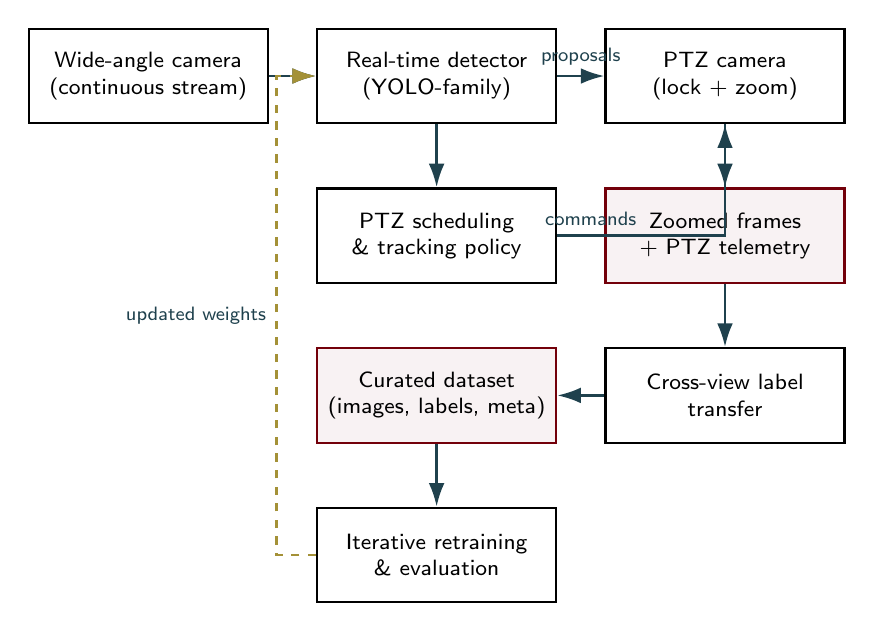
\begin{tikzpicture}[node distance=8mm and 6mm]
    % Nodes
    \node[flatblock] (widecam) {Wide-angle camera\\(continuous stream)};
    \node[flatblock, right=of widecam] (det) {Real-time detector\\(YOLO-family)};
    \node[flatblock, below=of det] (sched) {PTZ scheduling\\\& tracking policy};
    \node[flatblock, right=of det] (ptz) {PTZ camera\\(lock + zoom)};
    \node[data, below=of ptz] (ptzobs) {Zoomed frames\\+ PTZ telemetry};
    \node[flatblock, below=of ptzobs] (xfer) {Cross-view label\\transfer};
    \node[data, left=of xfer] (dataset) {Curated dataset\\(images, labels, meta)};
    \node[flatblock, below=of dataset] (train) {Iterative retraining\\\& evaluation};

    % Paths
    \draw[flatarrow] (widecam) -- (det);
    \draw[flatarrow] (det) -- node[above, labeltext]{proposals} (ptz);
    \draw[flatarrow] (det) -- (sched);
    \draw[flatarrow] (sched) -| node[above, labeltext, pos=0.1]{commands} (ptz);
    \draw[flatarrow] (ptz) -- (ptzobs);
    \draw[flatarrow] (ptzobs) -- (xfer);
    \draw[flatarrow] (xfer) -- (dataset);
    \draw[flatarrow] (dataset) -- (train);

    % Retrain loop
    \draw[flatarrow, dashed, color=CGold] (train.west) -- ++(-0.5,0) |- node[left, labeltext, pos=0.25]{updated weights} (det.west);
\end{tikzpicture}
\end{document}
